% cccc.tex
本節處理四邊固支 (CCCC) 邊界條件，即 $w = 0$ 且 $\psi_x = \psi_y = 0$ 於所有邊界。固支板無閉合形式解析解，故以文獻中 Ritz 法收斂值作為基準。

\subsection{基準解}
採用 Leissa (1969) 針對 Kirchhoff 板（薄板極限）給出的前六階無因次頻率參數 $\lambda^2 = \omega a^2 \sqrt{\rho h / D}$，對於極薄板 ($h/b=0.001$) 可視為 Mindlin 板的精確參考值：
\begin{align}
\lambda^2 &= [35.992,\; 73.413,\; 73.413,\; 108.27,\; 131.64,\; 132.24]
\end{align}
對應模態形狀依次為 (1,1), (2,1), (1,2), (2,2), (3,1), (1,3)。

\subsection{數值方法}
與簡支情況相同，以有限元素法配合懲罰法施加邊界條件，其中 $w$ 與 $\psi$ 的懲罰剛度均設為 $10^8 D$。積分策略同上。

\subsection{誤差定義}
誤差計算同式~\eqref{eq:error}，但此時 $w_{h,\text{exact}}$ 改為基準解 $\lambda^2$。

\subsection{結果}
圖~\ref{fig:cccc_modes} 顯示固支板前六階模態的收斂行為。

\begin{figure}[H]
\centering
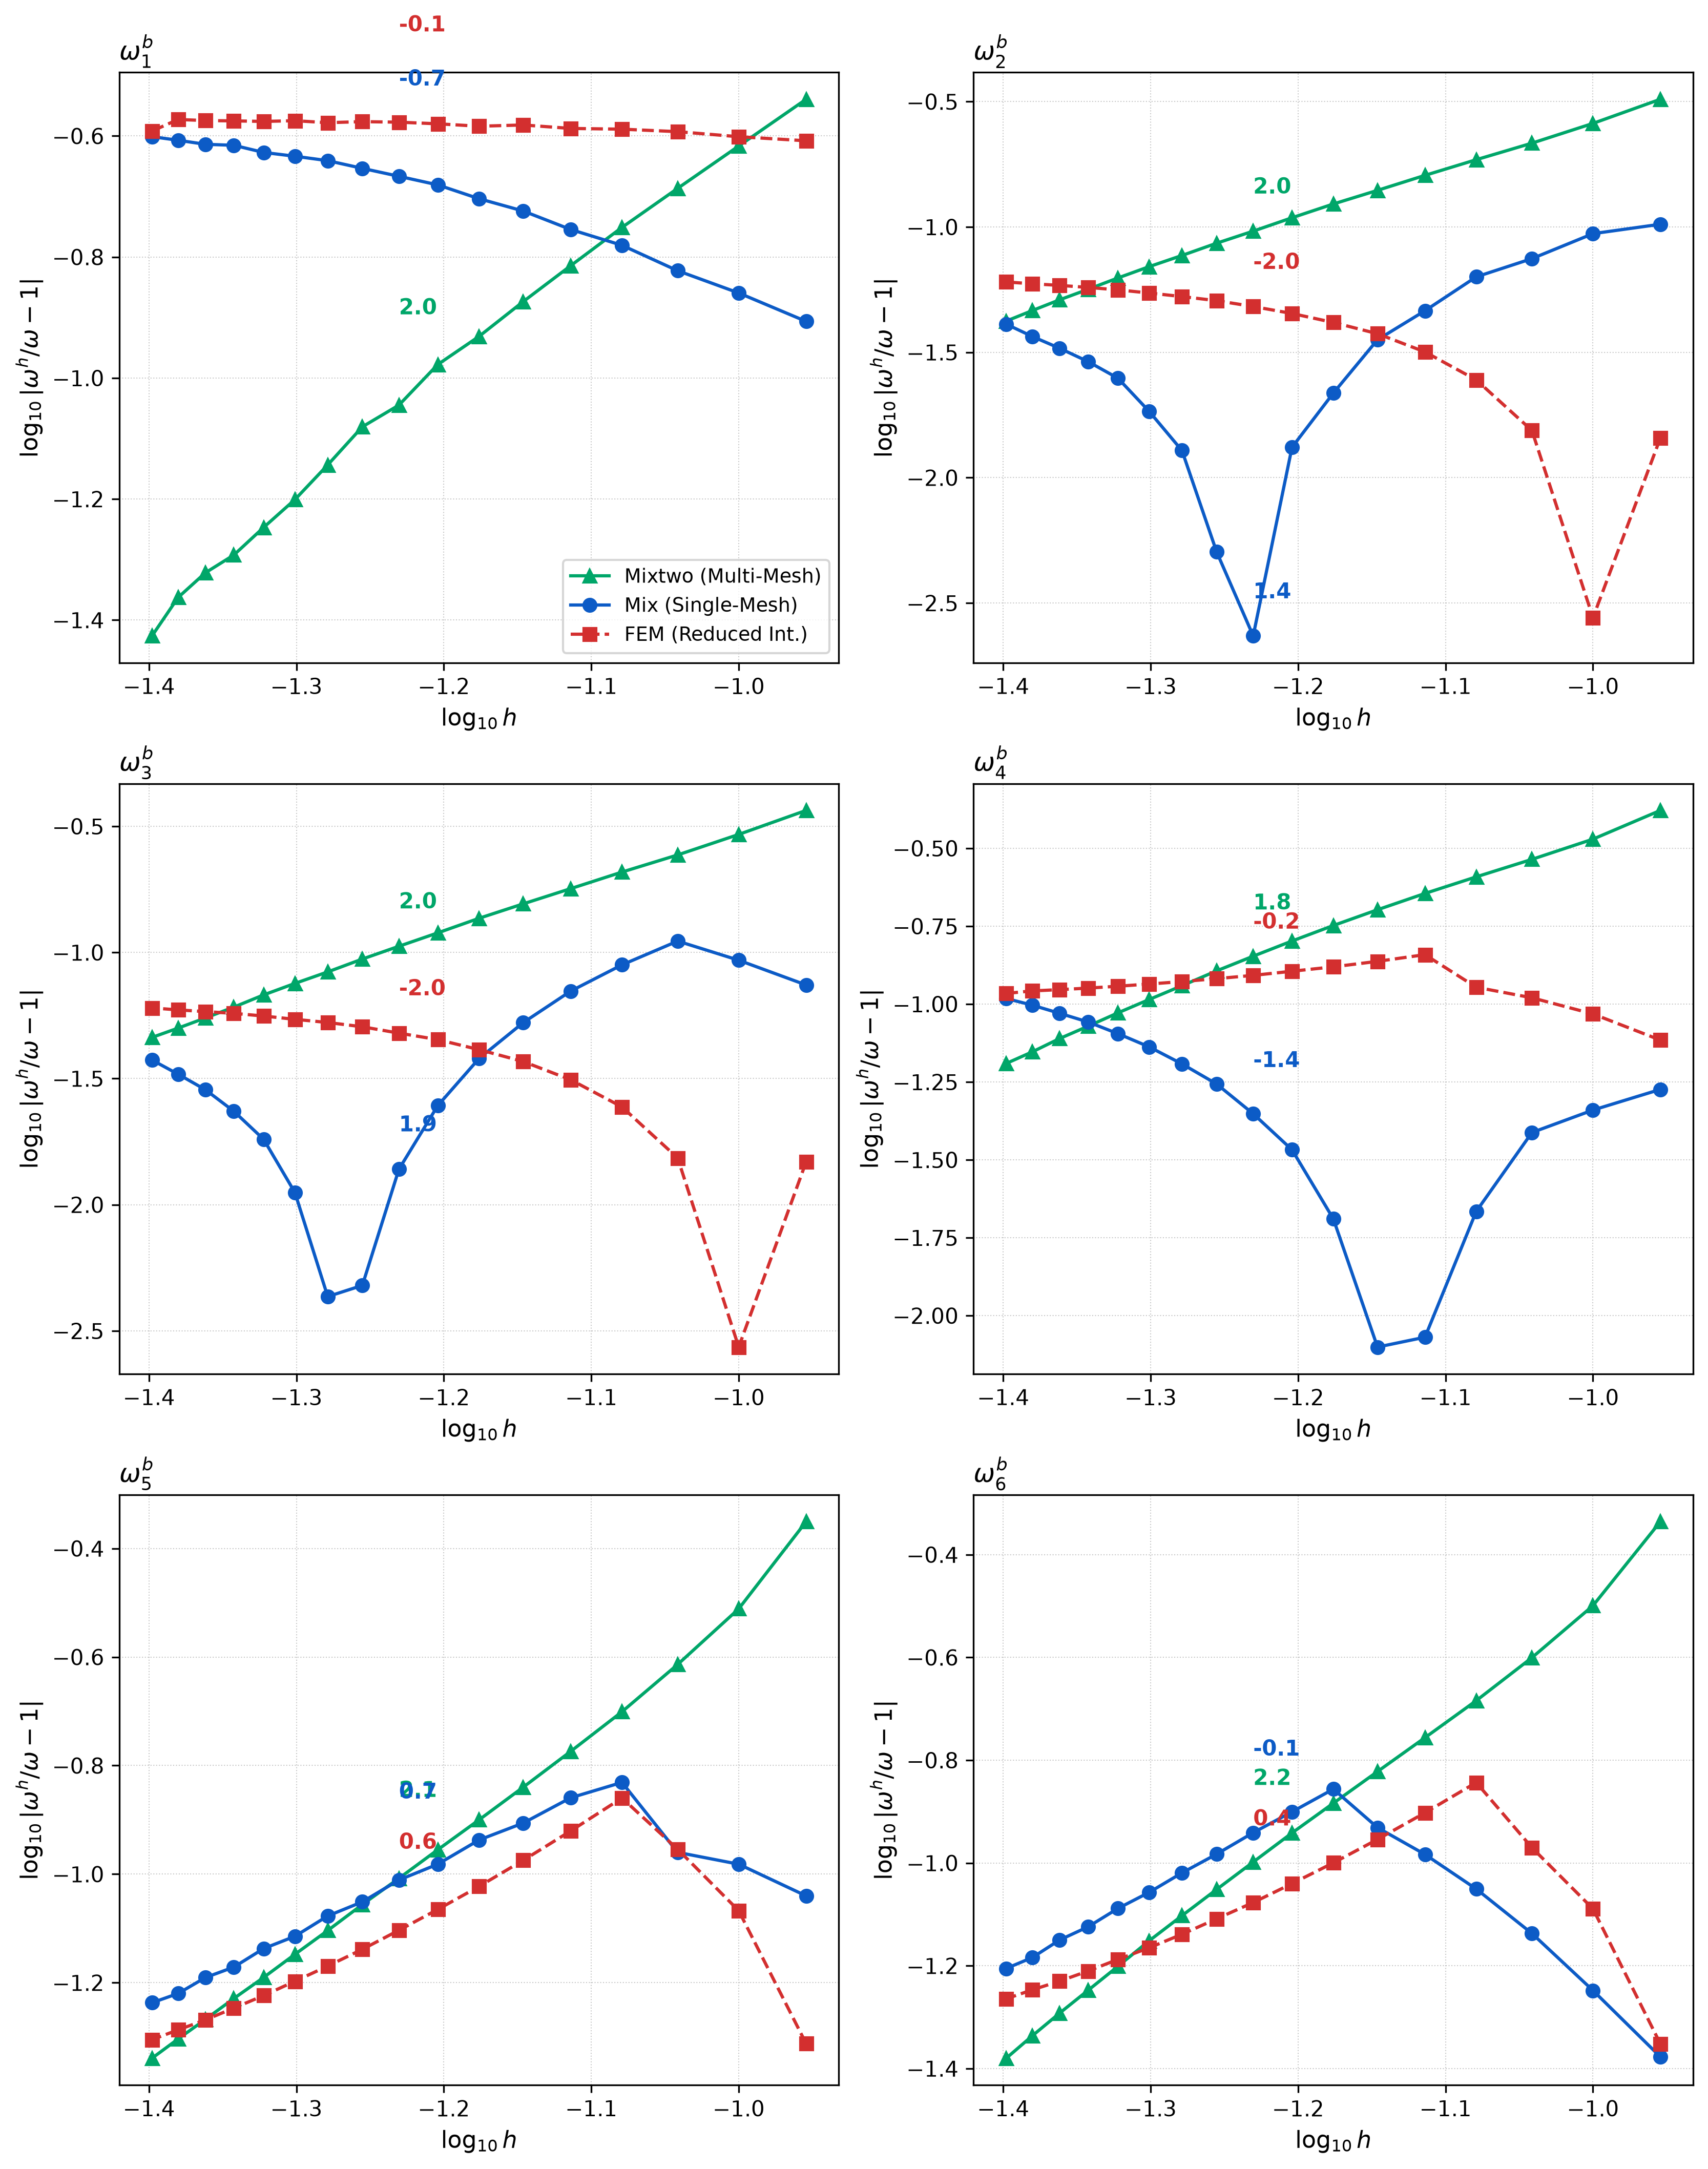
\includegraphics[width=\textwidth]{mode_6plots_4c.png}
\caption{四邊固支 Mindlin 板前六階模態收斂圖。上排：無因次頻率 $w_h$；下排：$\log_{10}$ 相對誤差。}
\label{fig:cccc_modes}
\end{figure}

從結果可知，數值頻率隨網格加密迅速收斂至基準解。與簡支板相比，固支板的頻率明顯較高（因邊界旋轉約束提高剛度）。第一模態 $w_h \approx 36$，而簡支板第一模態 $w_h \approx 19.74$。

